\documentclass{article}

\usepackage{imports}

\title{\bfseries работа на паре \TeX'а}
\author{Михаил Ушаков 7 мат}
\date{\today}

\begin{document}
\maketitle

\begin{itemize}
    \item[] \!\!\!\!\!\!\!\!Картинки
    \item[$\equiv$] Птички
    \item[$\equiv$] Типо квадратики...
\end{itemize}
    
\begin{figure}[t]
\begin{multicols}{2}
\hfill
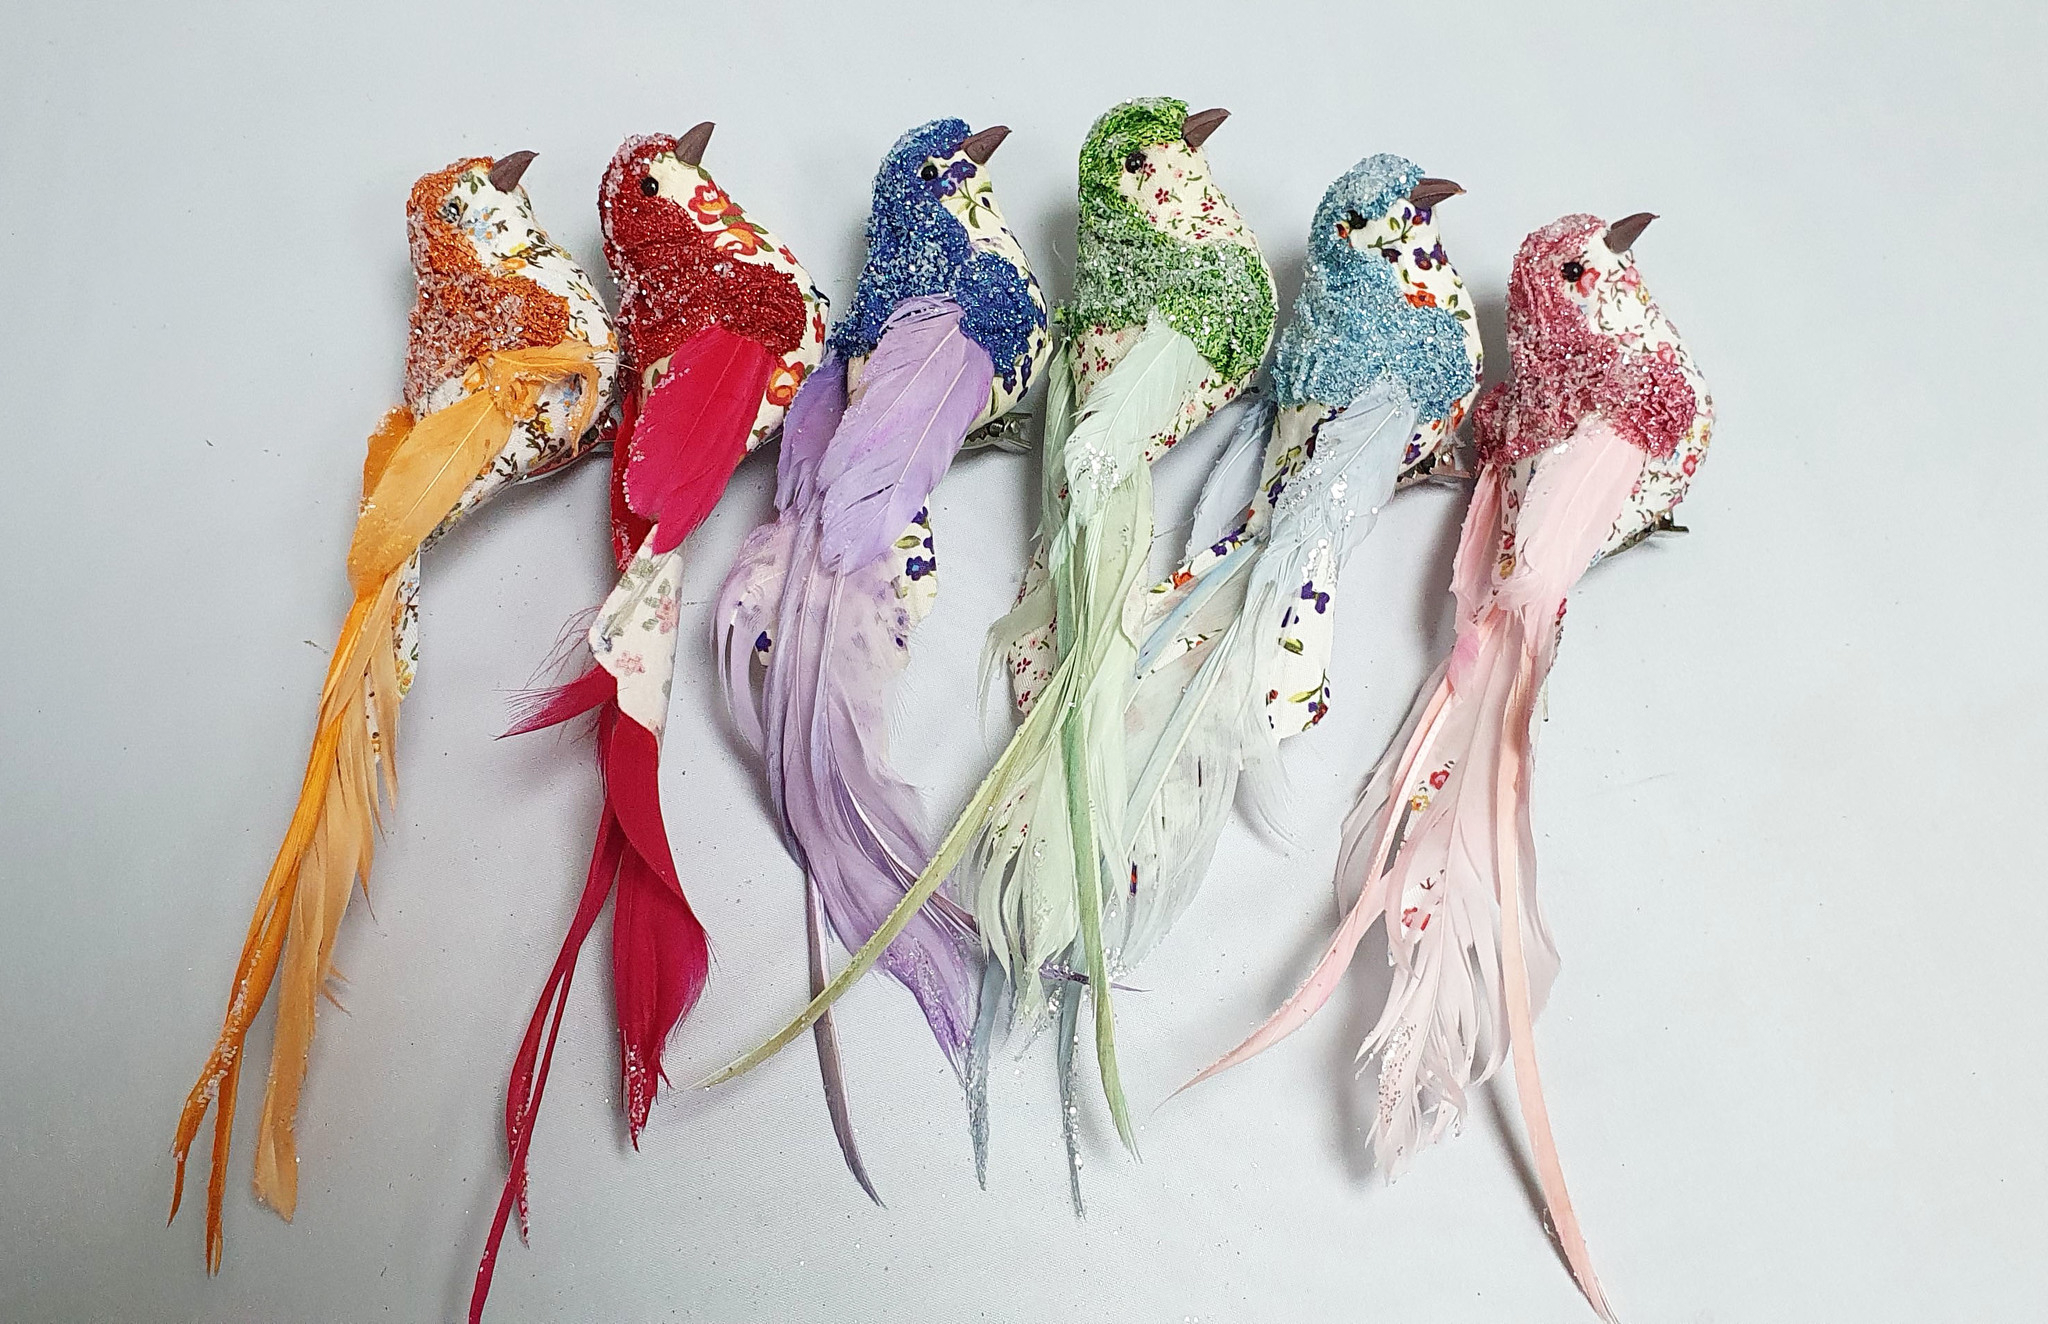
\includegraphics[width=7cm]{picture.jpg}
\hfill
\caption{Птички}
\label{figLeft}
\hfill
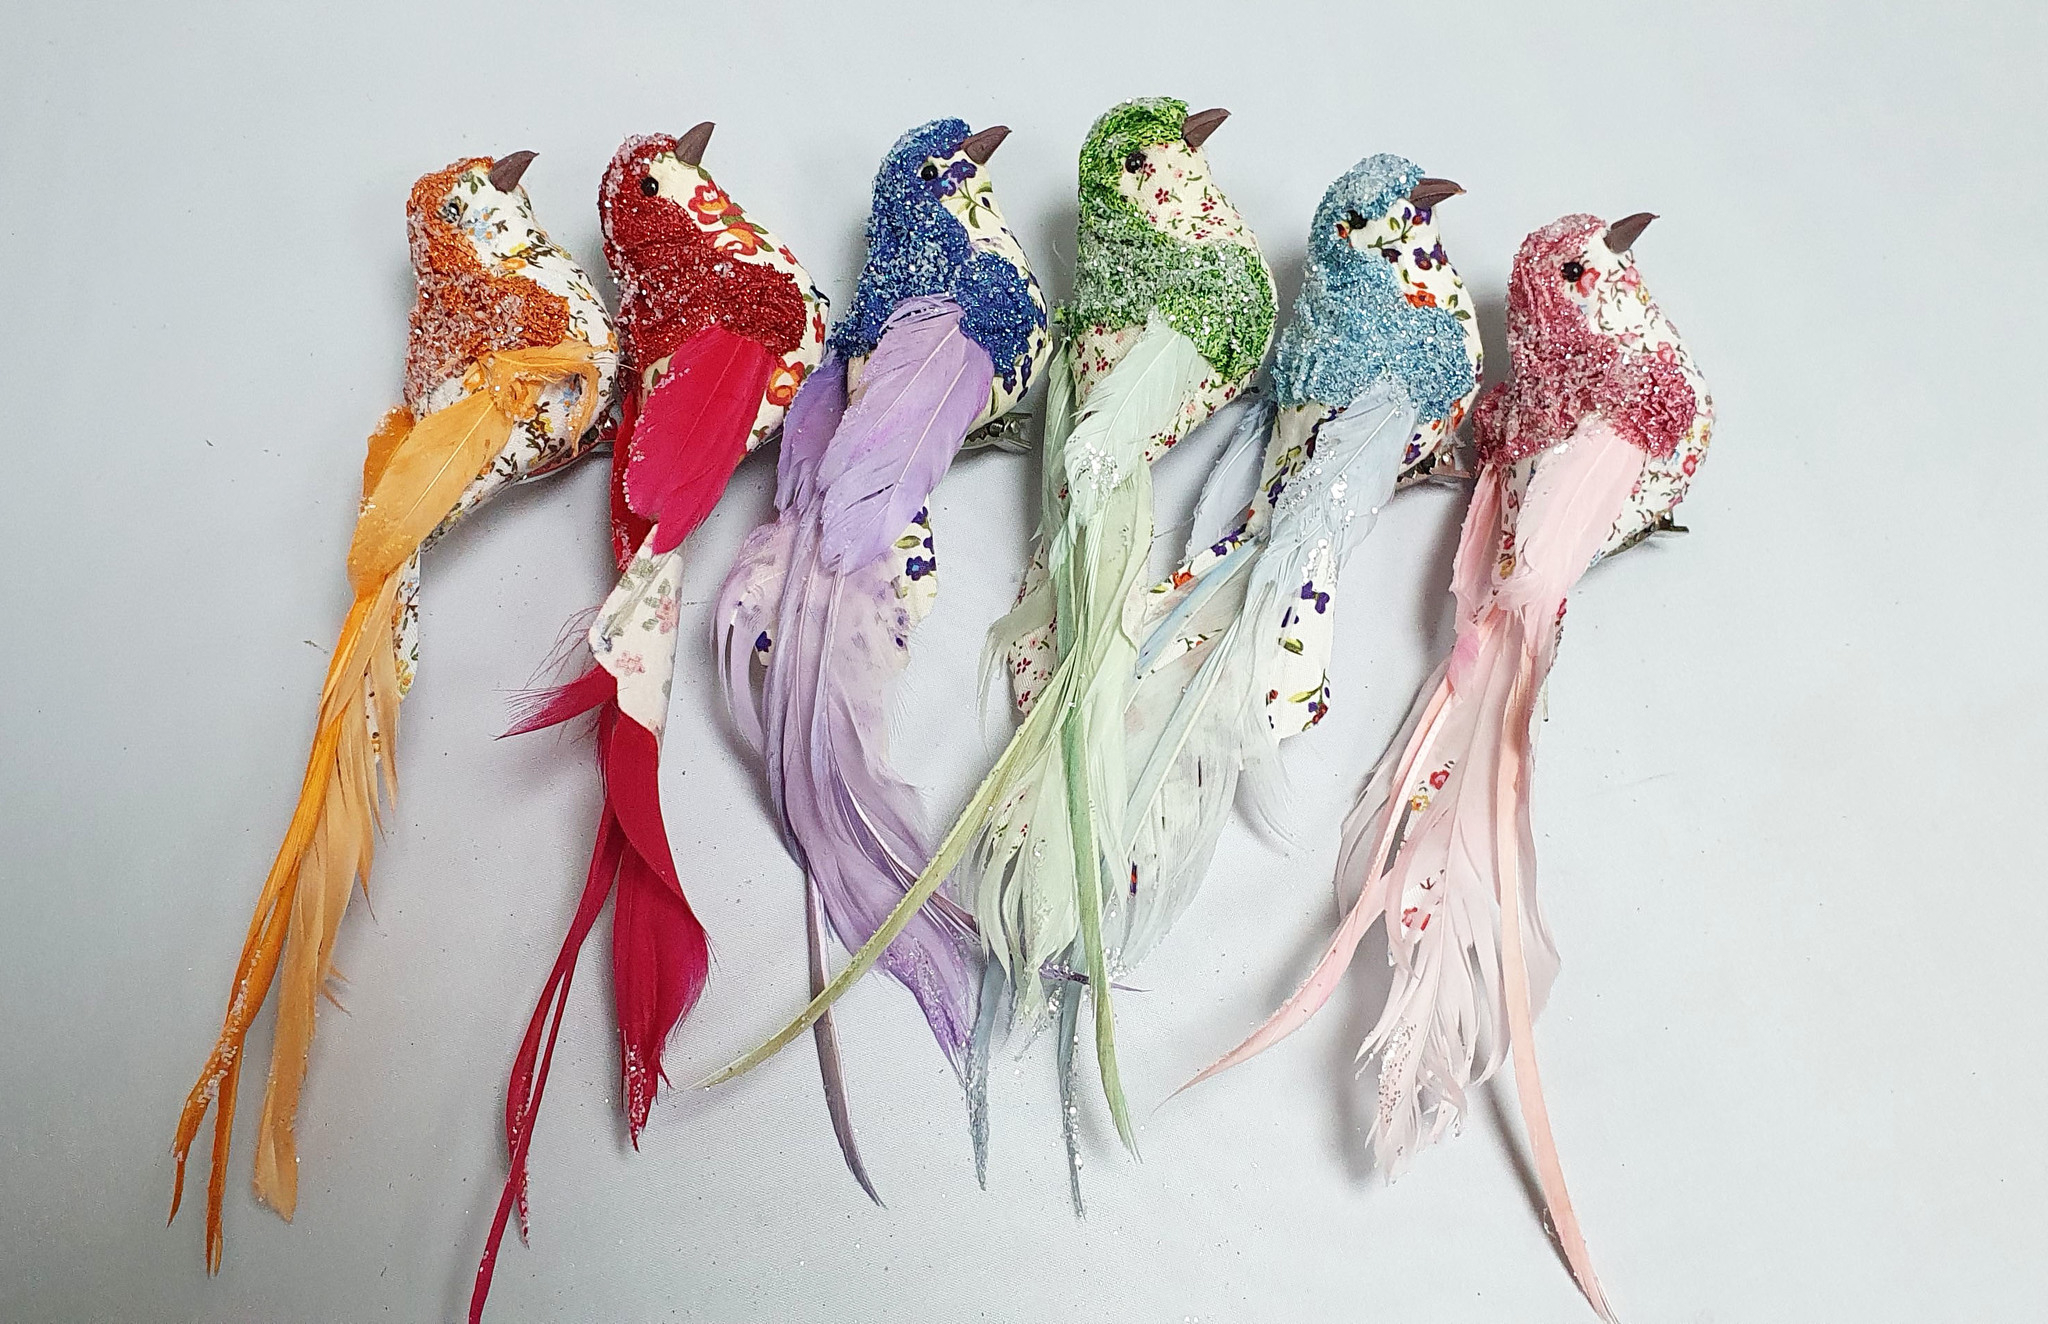
\includegraphics[width=7cm]{picture.jpg}
\hfill
\caption{Типо квадратики...}
\label{figRight}
\end{multicols}
\end{figure}

\end{document}